\section{Leading order analysis}
\label{section: thermodynamics leading order}


\begin{figure}[htb]
    \centering
    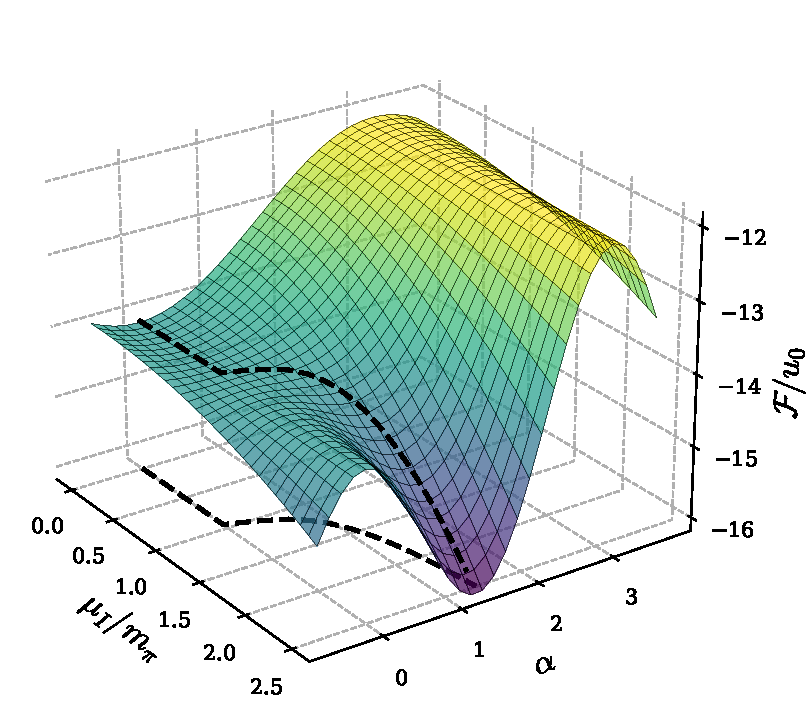
\includegraphics[width=0.9\textwidth]{../scripts/figurer/free_energy_surface.pdf}
    \caption{
        The surface is the free energy as a function of $\alpha$ and $\mu_I$.
        The black dashed lines illustrates the value of $\alpha$ which minimizes the free energy for a given value of $\mu_I$.
    }
    \label{fig: free energy surface}
\end{figure}

\todo[inline]{Være konsekvent: bruk kun fysiske eller bare masser/konstanter}
The leading order contribution to free energy is given by the static Lagrangian, to first order in Weinberg's power counting scheme.
We start by assuming $e = 0$, i.e., no electromagnetic interactions.
We thus get the leading order contribution to the free energy density from \autoref{static three-flavor Lagrangian}, and it is
%
\begin{equation}
    \Eff 
    = 
    - \frac{1}{2} f^2
    \left(
        \mu_I^2 \sin^2\alpha
        + 2\bar m^2 \cos\alpha
        + m_S^2
    \right).
\end{equation}
%
The parameter $\alpha$ is determined by minimizing $\Eff$ for a given value of $\mu_I$,
%
\begin{equation}
    \pdv{\Eff}{\alpha} = f^2 \left(\bar m^2 - \mu_I^2 \cos \alpha\right) \sin\alpha = 0.
\end{equation}
%
This gives an explicit formula for $\alpha$ in terms of $\mu_I$.
As long as the chemical potential is lower than the critical value $\mu_I^c = \bar m$, the only solution to this equation is $\alpha = 0$.
As the chemical potential reaches this critical value, the system undergoes a phase transition from the vacuum phase to the \emph{pion condensate} phase.
In this new phase, the solution is
%
\begin{align}
    \label{alpha as function of mu lowest order}
    \cos \alpha = \frac{\bar m^2}{\mu_I^2}.
\end{align}
%
We introduce a dimensionless variable $x^2 = \cos\alpha = \bar m^2 / \mu_I^2$.
This variable has the domain $[0, 1]$, and $\cos \alpha = x^2$ implies that $\sin^2 \alpha = 1 - x^4$.
Substituting the dimensionless variable into the free energy density, we get 
%
\begin{equation}
    \Eff = - \frac{u_0}{2} \left( x^2 + \frac{1}{x^2} \right) +\const
\end{equation}
%
We have introduced the characteristic energy density $u_0 = \bar m^2 f^2$.
This process of minimizing free energy for a given $\mu_I$ is illustrated in \autoref{fig: free energy surface}.



As we found in the last section, the pressure is given by negative the free energy density. 
We normalized the pressure to $\mu_I = \bar m$, or $x = 1$, and choose $p_0 = u_0$, so the dimensionless pressure is
%
\begin{equation}
    \label{pressure leading order chpt}
    \tilde p = -\frac{1}{p_0} \left(\Eff - \Eff_{x=1}\right) 
    % = \frac{1}{2} \left( x^2 + \frac{1}{x^2} - 2 \right).
    = \frac{1}{2} \left(x - \frac{1}{x}\right)^2.
\end{equation}
%
The charge density corresponding to a chemical potential is given by minus the derivative of the free energy with respect to that chemical potential. 
We must, however, not assume any dependence of $\alpha$ on $\mu_I$ when taking this derivative.
The isospin density is
%
\begin{equation}
    \label{isospin density}
    n_I = -\pdv{\Eff}{\mu_I} = f^2 \mu_I \sin^2 \alpha 
    = 
    \frac{u_0}{\mu_I} \left(\frac{1}{x^2} - x^2\right),
\end{equation}
%
while the strangeness is zero.
With this, the dimensionless energy density at $T = 0$ is
%
\begin{equation}
    \label{energy density leading order chpt}
    \tilde u = - \tilde p + \frac{\mu_I n_I}{u_0}
    = \frac{1}{2} \left( 2 + \frac{1}{x^2} - 3 x^2\right).
\end{equation}
%
The ratio of pressure to energy density is
%
\begin{equation} 
    \label{pressure energy ratio leading order chpt}
    \frac{p}{u} = \frac{1- x^2}{1+3x^2},
\end{equation}
%
which matches earlier results~\autocite{sonQCDFiniteIsospin2001}.
In the ultrarelativistic limit, where $\mu_I \rightarrow \infty$ and thus $x \rightarrow 0$, we get $p / u = 1$, or $u_\text{ur} = p$.
The non-relativistic limit is $\mu_I^2 = m_\pi^2(1 + \epsilon)$ and thus $x^{-2} = 1 + \epsilon$, $\epsilon \ll 1$.
With this we get $\tilde p = \epsilon^2 / 2 $, and $\tilde u = 2\epsilon$, so the equation of state is $\tilde u_\text{nr} = \sqrt 8 \sqrt{\tilde p}$.
The isospin density, and thus the pion number density, is $n_I = 2 \frac{u_0}{\bar m} \epsilon$, and we can therefore write the energy density in this limit as $u = \bar m n_I + \Oh(\epsilon^2)$.
The energy density is thus dominated by the rest mass as $\epsilon \rightarrow 0$, as we expect from the non-relativistic limit.
\autoref{fig: equation of state pions} shows the equation of state in two different regimes and compares it with the ultrarelativistic and non-relativistic limits.

\begin{figure}[!htb]
    \centering
    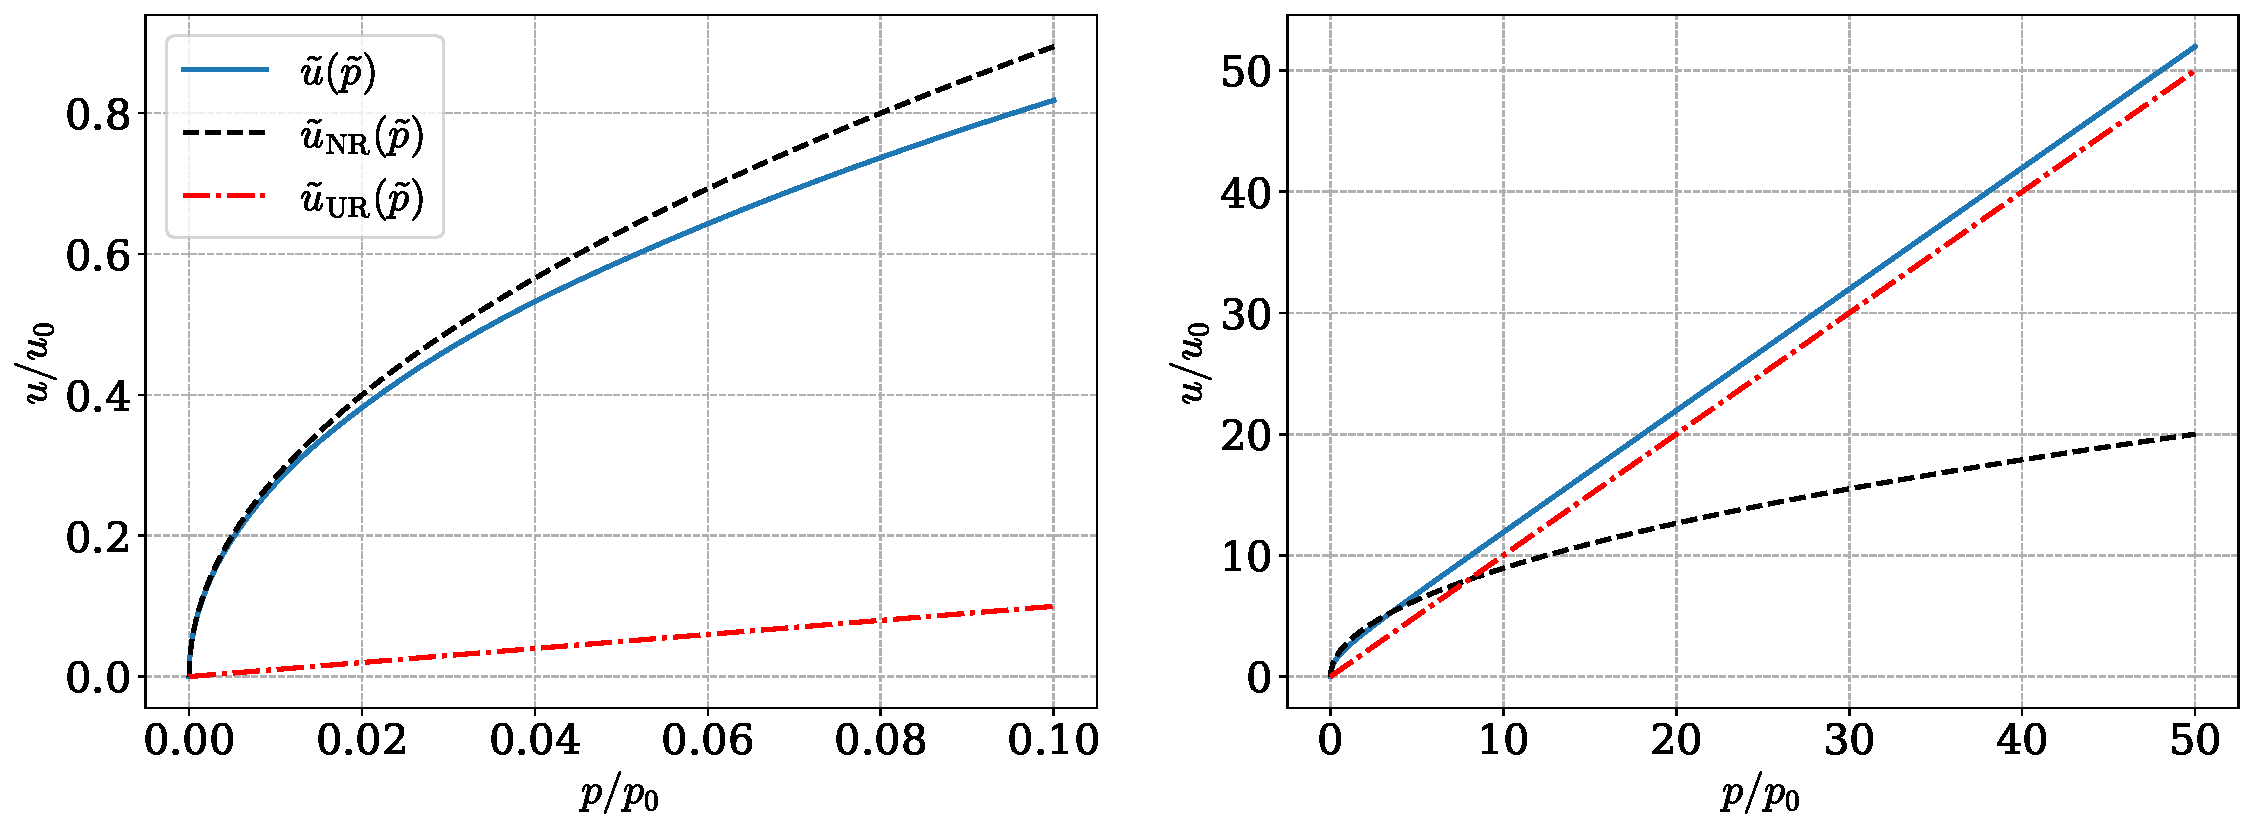
\includegraphics[width=0.95\textwidth]{../scripts/figurer/pion_star/pion_eos.pdf}
    \caption{
        The leading order equation of state from two-flavor chiral perturbation theory, in two different regimes.
        The full equation is shown as a solid line and is compared to the ultrarelativistic and non-relativistic limits shown as dashed lines. 
        The $y$-axis shows the energy density normalized to $u_0$, $x$-axis shows the pressure normalized to $p_0$.
        We have chosen $p_0 = u_0$.
    }
    \label{fig: equation of state pions}
\end{figure}



\subsection{Including electromagnetism}
\label{subsection: including electromagnetism lo eos}


From \autoref{static Lagrangian three-flavor EM}, the free energy density, including electromagnetic interactions, is
%
\begin{equation}
    \Eff =
    - \frac{1}{2} f^2
    \left(
        \mu_I^2 \sin^2\alpha + 2 \bar m^2\cos\alpha 
        + \Delta m_\text{EM}^2\cos^2\alpha
        - \frac{1}{3}\Delta m_\text{EM}^2 + m_S^2
    \right).
\end{equation}
%
Free energy minimization now gives
%
\begin{equation}
    \frac{1}{u_0}\pdv{\Eff}{\alpha}
    = 
    \left[ \left( \frac{1}{x^2} - \Delta \right) \cos \alpha - 1\right] \sin \alpha = 0.
\end{equation}
%
Here, $x$ is defined as before, and we introduced the new quantity $\Delta = \Delta m_{\text{EM}}^2 / \bar m^2= 0.06916$.
We see that the phase transition is raised, the critical chemical potential is now $\mu_I^c = \bar m \sqrt{1 + \Delta}$, the mass of the charged pions.
Below this value, $\alpha = 0$ remains the only solution.
In the pion condensate phase, the solution is
%
\begin{equation}
    \cos \alpha = \frac{\bar m^2}{\mu_I^2 - \Delta m_\text{EM}^2}
    = \frac{1}{\frac{1}{x^2} -  \Delta}.
\end{equation}
%
This reduces to our old solution for $\Delta = 0$, as it should.
With the same procedure as in the last section, we get the pressure and energy density
%
\begin{align}
    \label{pressure with em interaction}
    \tilde p_\text{EM}
    & = \frac{1}{2} 
    \left(
        \frac{1}{x^2} - \Delta
        + \frac{x^2}{1 - x^2 \Delta} 
        - 2 
    \right), \\
    % & = \frac{1}{2} 
    % \left(
    %     \sqrt{\frac{1}{x^2} - \Delta}
    %     -\frac{1}{\sqrt{\frac{1}{x^2} - \Delta}} 
    % \right)^2, \\
    \tilde u_\text{EM}
    &= \frac{1}{2} 
    \left(
        \frac{1}{x^2} 
        - x^2 \frac{3 - x^2 \Delta }{(1 - x^2 \Delta)^2}
        + 2 + \Delta
    \right).
\end{align}
%
The ratio between pressure and energy is now
%
\begin{equation}
    \frac{p_\text{EM}}{u_\text{EM}} 
    = 
    \frac{
        1 - (2\Delta + 1)x^2 + \Delta(\Delta + 1)x^4
        }{
        1 + 3x^2 - \Delta (\Delta +1)x^4
        }.
\end{equation}
%
In the limit $\Delta = 0$, these results reduce to those we found in the last section.
In the ultra-relativistic limit, that is, for  $x \ll 1$, the behavior is the same as before, and we again approach $p = u$.
As the mass of the charged pions have changed, the non-relativistic limit is now obtained by substituting $x^{-2} = 1 + \Delta + \epsilon$, for $\epsilon \ll 1$.
To first order in $\epsilon$ we get $\tilde p = \epsilon / 2$, which is the same as before.
However, the energy density limit is perturbed by the inclusion of electromagnetism and is now $\tilde u = 2(1 + \Delta) \epsilon$.
The non-relativistic equation of state is thus still a polytrope of the form $\tilde p = K \tilde u^2$, however the constant is now $K^{-1} = 8 (1+\Delta)^2$.


\begin{figure}[!htb]
    \centering
    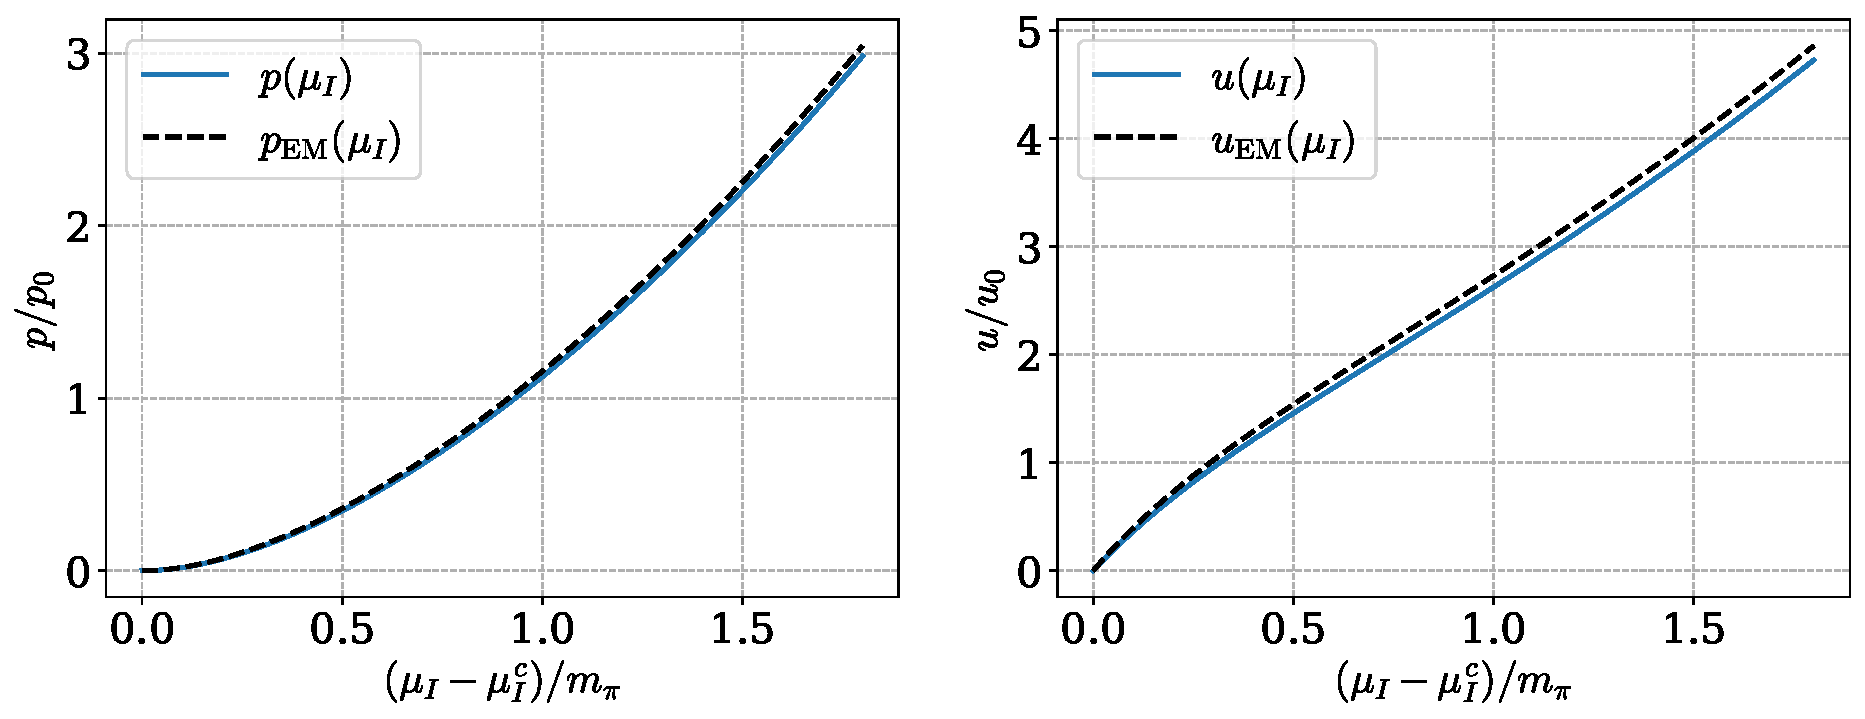
\includegraphics[width=0.95\textwidth]{../scripts/figurer/pion_star/pion_up.pdf}
    \caption{
        Left: The pressure, normalized to $p_0$, as a function of the chemical potential above the critical value, normalized to $\bar m$.
        Right: The energy density, normalized to $u_0$, also as a function of the chemical potential.
        Results with electromagnetic interaction are shown as dashed lines.
        The $y$-axis corresponds to different absolute values of isospin-chemical potential, as the critical value of the chemical is changed by the inclusion of electromagnetic interactions. See main text for details.
        }
        \label{fig: pressure and energy with EM interaction}
\end{figure}



\begin{figure}[!htb]
    \centering
    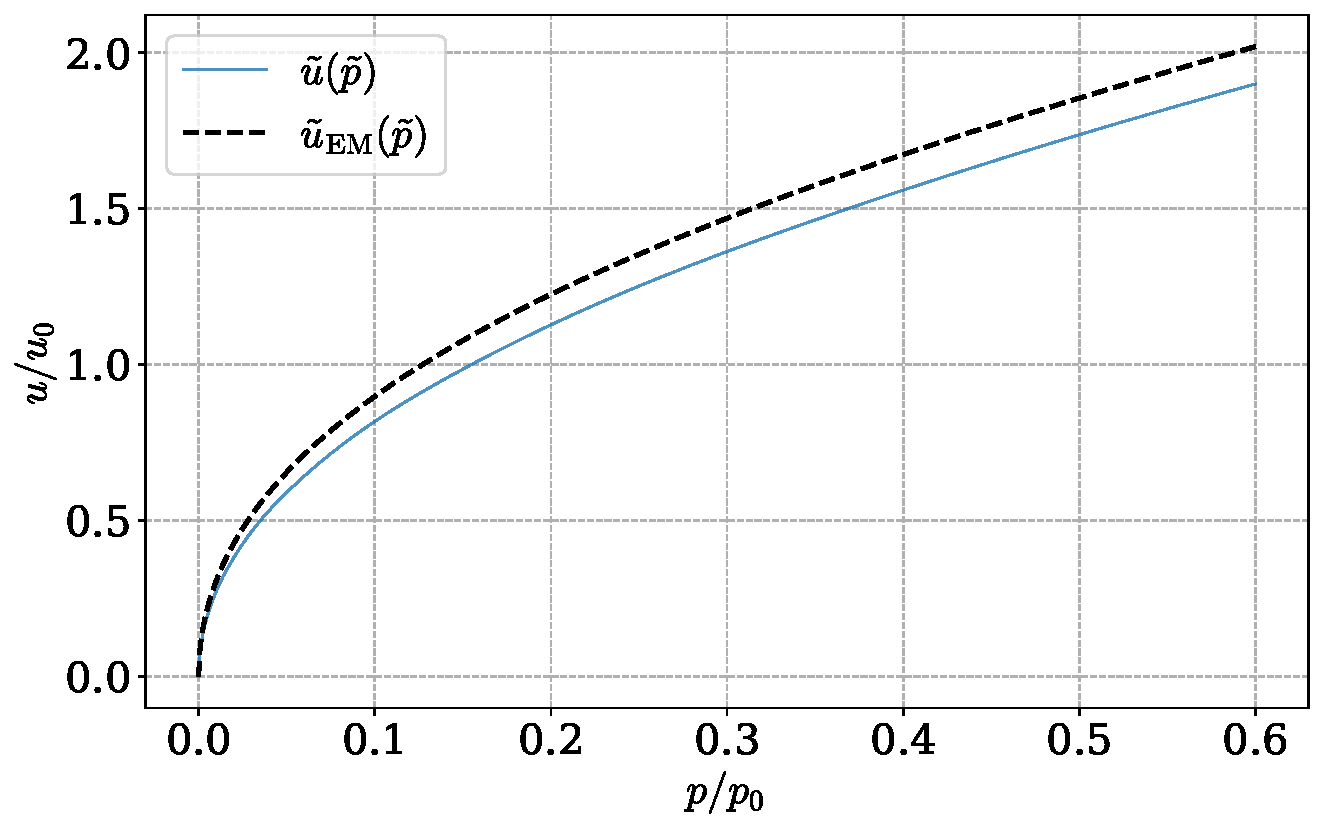
\includegraphics[width=0.65\textwidth]{../scripts/figurer/pion_star/pion_eos_EM.pdf}
    \caption{
        The equation of state in the pion condensate phase. 
        Results with electromagnetic interactions are shown as dashed lines.
        The energy density and pressure is normalized to $u_0$ and $p_0 = u_0$.
        }
    \label{fig: eos chpt em interaction}
\end{figure}





\section{Phase transitions}

As the static Lagrangian has the same form in the kaon condensed phase as in the pion condensed phase, the analysis of the phase transition and $\alpha$ as a function of $\mu_\Kpm$ will be the same as in the pion condensate.
The system will be in the phase whose static Lagrangian minimizes the free energy, or equivalently, maximizes the pressure.
Therefore, we can find the transition line between the condensates by setting the pressure of the two condensates equal.
Using \autoref{pressure leading order chpt}, and the similar expression in the kaon condensed phase, we get
%
\begin{equation}
    p 
    = \frac{1}{2} f^2 m_\Kpm^2 \left( \frac{\mu_\Kpm}{m_\Kpm} - \frac{m_\Kpm}{\mu_\Kpm} \right)^2
    =
    \frac{1}{2} f^2m_\pi^2  \left( \frac{\mu_I}{m_\pi} - \frac{m_\pi}{\mu_I} \right)^2.
\end{equation}
%
Solving for $\mu_\Kpm$, we get
%
\begin{equation}
    \label{transition line pion and charged condensates}
    \mu_\Kpm =\frac{1}{2\mu_I} \left(\mu_I^2 - m_\pi^2  + \sqrt{(\mu_I^2 - m_\pi^2)^2 + 4\mu_I^2 m_\Kpm^2}\right).
\end{equation}
%
The transitions into the condensates are at $\mu_I = m_\pi$, and $\mu_\Kpm = m_\Kpm$.
This point, $(\mu_I, \mu_S) = (m_\pi, m_\Kpm - m_\pi/2)$, satisfies \autoref{transition line pion and charged condensates}, and is thus a triple point between the vacuum phase, $\pipm$ condensate and the $\Kpm$ condensate. 
Similarly, the line between the charged and neutral kaon condensed phase is defined by
%
\begin{equation}
    \frac{1}{2} f^2 m_\Kpm^2 \left( \frac{\mu_\Kpm}{m_\Kpm} - \frac{m_\Kpm}{\mu_\Kpm} \right)^2
    =
    \frac{1}{2} f^2 m_\Ko^2 \left( \frac{\mu_\Ko}{m_\Ko} - \frac{m_\Ko}{\mu_\Ko} \right)^2.
\end{equation}
%
The solution is
%
\begin{equation}
    2 \mu_\Kpm 
    = \frac{1}{\mu_\Ko}
    \left(
        \mu_\Ko^2 - m_\Ko^2  + \sqrt{(\mu_\Ko^2 - m_\Ko^2)^2 + 4\mu_\Ko^2m_\Kpm^2}
    \right).
\end{equation}
%
We can expand this to first order in the difference in mass between the kaons, $m_\Ko^2 - m_\Kpm^2 = \Delta m^2$, which gives
%
\begin{align}
    \nonumber
    \mu_\Kpm
    &= \frac{1}{\mu_\Ko} 
    \left(
        \mu_\Ko^2 - m_\Ko^2 + \sqrt{(\mu_\Ko^2 + m_\Ko^2)^2 + 4\mu_\Ko^2 \Delta m^2}
    \right)\\
    &= \mu_\Ko \left(1 + \frac{\Delta m^2}{\mu_\Ko^2 + m_\Ko^2}\right)
    + \Oh\left( \frac{\Delta m^4}{ (\mu_\Ko^2 + m_\Ko^2)^2} \right)
\end{align}
%
This is an excellent approximation, as $\Delta m^4 / 4 m_\Ko^4 \approx 4 \times 10^{-4}$.
The triple point is in this case at $\mu_\Kpm = m_\Kpm$, $\mu_\Ko = m_\Ko$ or $(\mu_I, \mu_S) = (m_\Kpm - m_\Ko, [m_\Kpm+m_\Ko]/2)$.
If we consider $\Delta m = 0$, then this reduces to $ \mu_\Kpm = \mu_\Ko$, or $\mu_S = 0$, as obtained in~\autocite{kogutQCDSmallNonzero2001}.
A similar analysis gives the transition line between all phases.
\autoref{fig: phase diagram} shows the phase diagram in the $\mu_I-\mu_S$-plane.

\begin{figure}[!htb]
    \centering
    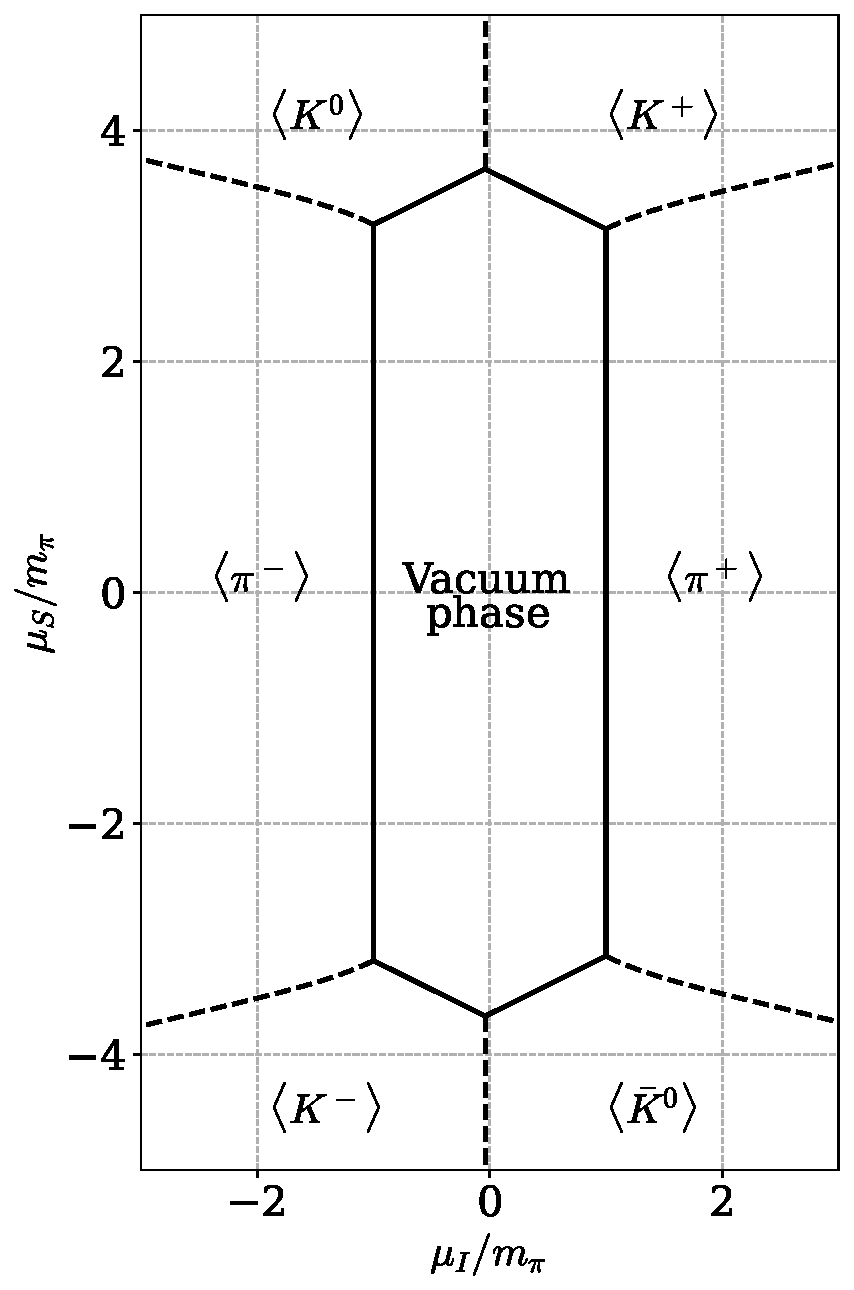
\includegraphics[width=0.5\textwidth]{../scripts/figurer/phase_diagram.pdf}
    \caption{
        Phase diagram of \chpt\ in the $\mu_I-\mu_S$-plane.
        Chemical potentials are given in units of then pion mass.
        The expectation values in each region indicate which particles form a condensate.
        The dashed lines are first-order phase transitions between the condensates, while the solid line indicates the second-order phase transition from the vacuum phase of the vacuum to the condensates.
        }
    \label{fig: phase diagram}
\end{figure}

In the pion phase, the isospin and strangeness densities are
%
\begin{equation}
    n_I = - \pdv{\Eff}{\mu_I} = f_\pi^2 \mu_I \left( 1 - \frac{m_\pi^4}{\mu_I^4} \right), \quad
    n_S = - \pdv{\Eff}{\mu_S} = 0.
\end{equation}
%
In the charged kaon condensed phase, they are
%
\begin{equation}
    n_I = - \pdv{\Eff}{\mu_I} 
    = \frac{1}{2} \pdv{\Eff}{\mu_\Kpm}
    = \frac{1}{2} f^2_\pi \mu_\Kpm \left( 1 - \frac{m_\Kpm^4}{\mu_\Kpm^4} \right), \quad
    n_S = - \pdv{\Eff}{\mu_S} = f_\pi^2 \mu_\Kpm  \left( 1 - \frac{m_\Kpm^4}{\mu_\Kpm^4} \right).
\end{equation}
%
At the line of phase transition, $\mu_\Kpm > m_\Kpm$.
The strangeness density thus jumps discontinuously to a non-zero value.
This phase transition is, therefore, of first order.
In the neutral kaon condensed phase, the isospin density is
%
\begin{equation}
    n_I = - \pdv{\Eff}{\mu_I} 
    = -\frac{1}{2} \pdv{\Eff}{\mu_\Kpm}
    = - \frac{1}{2}  f^2_\pi \mu_\Kpm \left( 1 - \frac{m_\Kpm^4}{\mu_\Kpm^4} \right).
\end{equation}
%
This, too, will change discontinuously between the two kaon condensed phases.
Similar arguments hold between all condensates.
This indicates that the transitions between condensates are of \emph{first order}.



\subsection{Electromagnetic contribution}

We can describe the effect of electromagnetic interactions on the pressure, as obtained \autoref{subsection: including electromagnetism lo eos}, by modifying the isospin chemical potential by $\mu^2_I \rightarrow \mu^2_I - \Delta m_\text{EM}^2$.
From the structure of the Lagrangian \autoref{static Lagrangian three-flavor EM kaon}, the same will happen in the case of the charged kaon, only the change will be $\mu^2_\Kpm \rightarrow \mu^2_\Kpm - \Delta m_\text{EM}^2$, while from \autoref{static Lagrangian neutral kaon} we see that the results will be unchanged by electromagnetic interactions.
We define the effective chemical potential by ${\mu'}^2 = \mu^2 - \Delta m_\text{EM}^2$.
The transitions between the vacuum phase and the condensed phase will now be $\mu'_I = \bar m$ and $\mu_\Kpm' = m_\Kpm$, while the line between these condensed phases is now
%
\begin{equation}
    m_\Kpm^2
    \left(
         \frac{{\mu_\Kpm'}}{m_\Kpm}
         - \frac{m_\Kpm}{{\mu_\Kpm'}} 
        \right)^2
    =
    m_\pi^2  
    \left( 
        \frac{{\mu_I'}}{m_\pi}
        - \frac{m_\pi}{{\mu_I'}}
    \right)^2,
\end{equation}
%
The neutral kaon condensate, on the other hand, remains unchanged by the inclusion of electromagnetic interactions.
The line between the kaon condensates is thus given by
%
\begin{equation}
    m_\Kpm^2
    \left(
         \frac{{\mu_\Kpm'}}{m_\Kpm}
         - \frac{m_\Kpm}{{\mu_\Kpm'}^2} 
        \right)^2
    =
    m_\Ko^2  
    \left( 
        \frac{{\mu_\Ko}}{m_\Ko}
        - \frac{m_\Ko}{{\mu_\Ko}^2}  
    \right)^2.
\end{equation}
%
The new phase diagram is shown in \autoref{fig: phase diagram EM} in red, where it is compared with the results without electromagnetic interactions in black.
The change is very small. 
However, it affects the pion condensation more than the charged kaon.
This is because, as we discussed earlier, the \emph{square} of the mass is the same by Dashen's theorem, $\Delta m_\text{EM}^2$, while the absolute shift will depend on the ratio between $\Delta m_\text{EM}$ and the non-electromagnetic mass.
This is thus lower for the heavier kaon.
The line between the kaon condensates is moved slightly closer to $\mu_I = 0$, as the electromagnetic contribution to the lighter charged kaon mass reduces the difference between its and the neutral kaon's mass.

\begin{figure}[!htb]
    \centering
    \begin{subfigure}{0.49\textwidth} 
        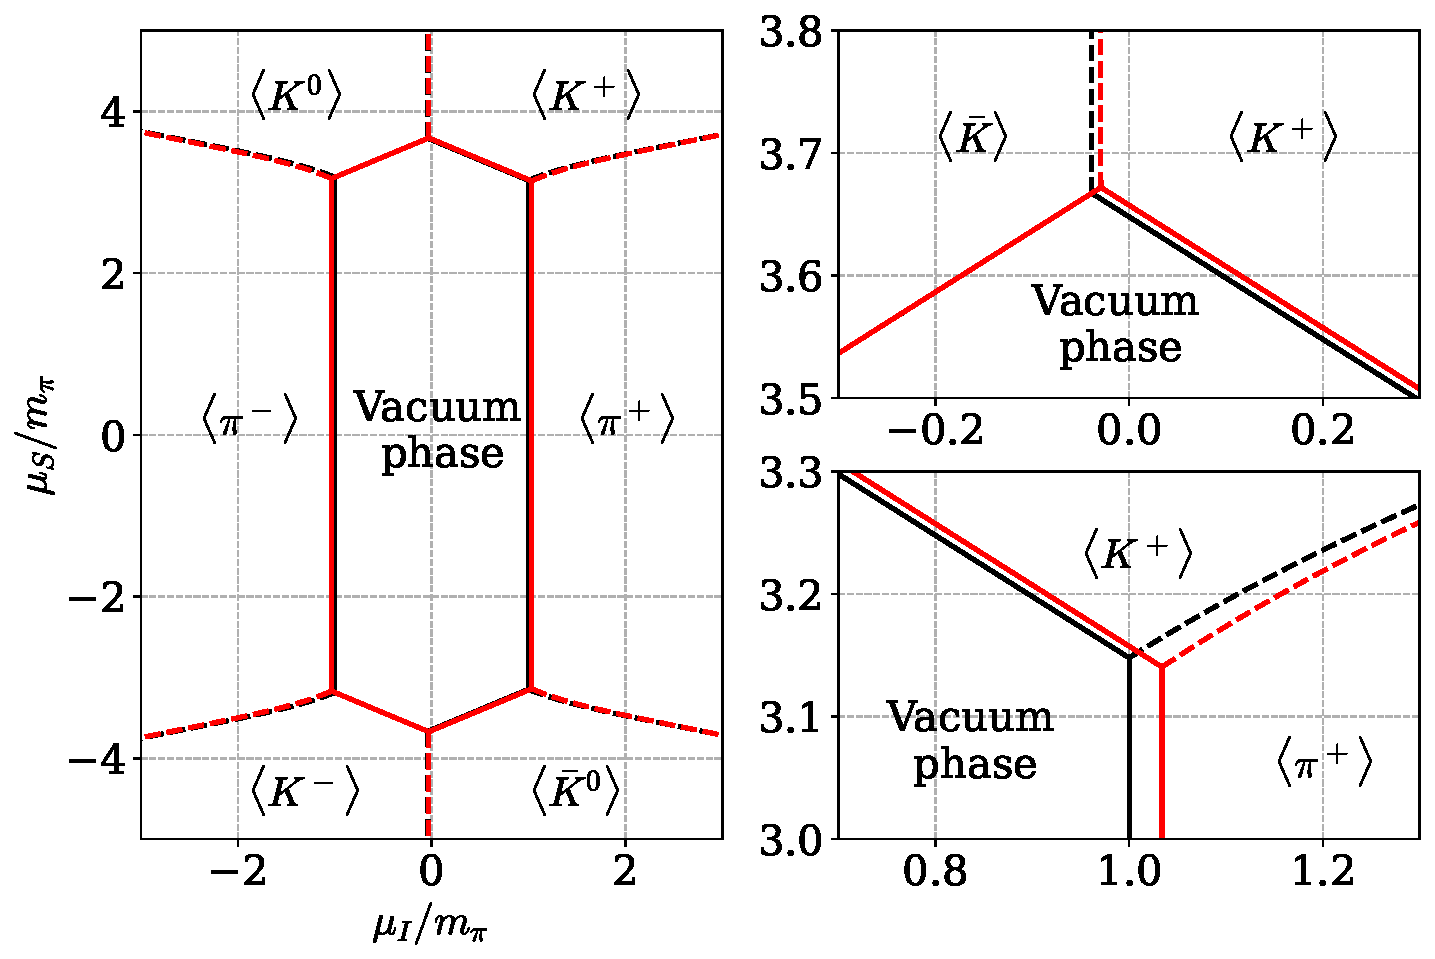
\includegraphics[width=\textwidth]{../scripts/figurer/phase_diagram_EM.pdf}
    \end{subfigure}
    \begin{subfigure}{0.49\textwidth}
        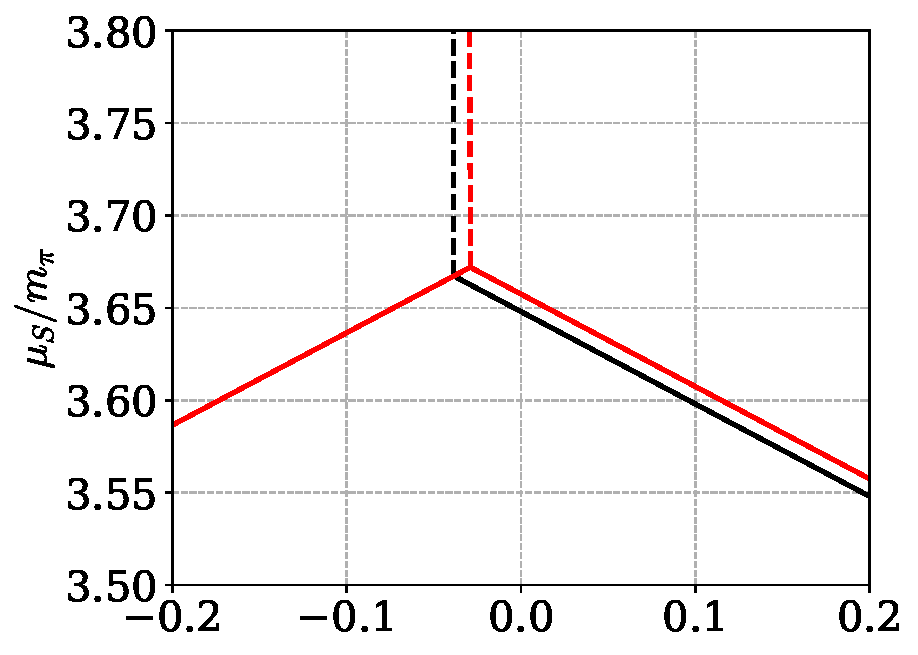
\includegraphics[width=\textwidth]{../scripts/figurer/phase_diagram_EM3.pdf}
        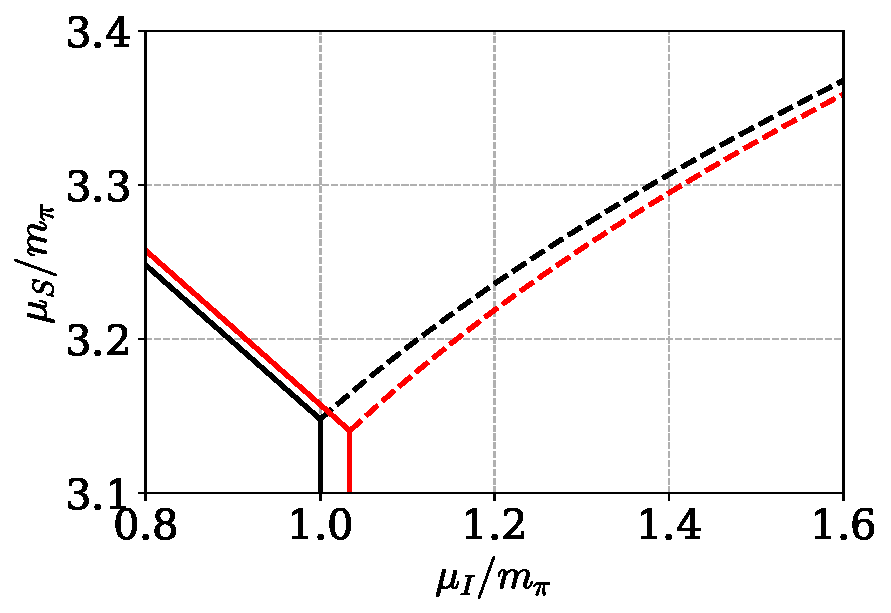
\includegraphics[width=\textwidth]{../scripts/figurer/phase_diagram_EM2.pdf}
    \end{subfigure}
    \caption{
        The phase diagram of \chpt\ in the $\mu_I-\mu_S$-plane.
        The black lines are results without the electromagnetic interactions, while red lines are results including them. 
        To the right, we have zoomed in on two of the triple points.
        At the top is the intersection of the normal, neutral kaon condensed and charged kaon condensed phases, while at the bottom is the intersection of the normal, pion condensed, and charged kaon condensed phases.
        }
    \label{fig: phase diagram EM}
\end{figure}



